
%Document Class Definition
\documentclass{article}

%Required Packages
\usepackage{xcolor}
\usepackage[utf8]{inputenc}
\usepackage[french]{babel}
\usepackage{amsfonts}
\usepackage{amssymb}
\usepackage[T1]{fontenc}      % LaTeX
\usepackage{fontawesome}
\usepackage{tikz}
	\usetikzlibrary{babel} %correction for the french version of the document with XeLaTeX
	\usetikzlibrary{shapes.geometric}
	\usetikzlibrary{calc}
	\usetikzlibrary{decorations.pathreplacing}
\usepackage[left=1cm,right=1cm,top=1cm,bottom=1cm]{geometry}
\usepackage{setspace}
\usepackage[absolute,overlay]{textpos}
\usepackage{hyperref}
\usepackage{tabularx}
\usepackage{calc}
\usepackage{ifthen}
\usepackage{coolstr}
\usepackage{coolstr}
\usepackage{textcase}
\usepackage{amsmath}
\usepackage{relsize}
\usepackage{moresize}
\usepackage{times}
\usepackage{enumitem}
\usepackage{booktabs}
\usepackage{multirow}
\usepackage{colortbl}
\usepackage{mathabx}
\usepackage{graphicx}
  	  	\graphicspath{{./fig/}} %fig path
  	  	
%Definition of the colors
\definecolor{white}{RGB}{255,255,255}
\definecolor{sidecolor}{RGB}{200,200,200}
\definecolor{mainblue}{RGB}{0,70,153}
\definecolor{maingray}{RGB}{144,144,144}

%Define CV Variables
\newcommand{\cvfirstname}{Loïc}
\newcommand{\cvlastname}{Van Hoorebeeck}
\newcommand{\cvtitle}{Engineer in Applied Mathematics}

\newcommand{\cvemail}{loicvanhoorebeeck@gmail.com}
\newcommand{\cvphonenumber}{(+32) 475.36.75.28}
\newcommand{\cvaddress}{17, rue de l'Argentine 1310 La Hulpe}
\newcommand{\cvlocation}{1310 La Hulpe, Belgium}
\newcommand{\cvlinkedin}{https://www.linkedin.com/in/loïc-van-hoorebeeck-96512113b/}
\newcommand{\github}{https://github.com/loicvh}
\newcommand{\Web}{https://davebulaval.github.io}

%Command for vertical centering of text into tabular
\renewcommand{\tabularxcolumn}[1]{m{#1}}

%Command for horizontal centering of specified width into tabular
\newcolumntype{M}[1]{>{\centering\arraybackslash}m{#1}}

%Command for bold font and textcolor to apply to a specific column into tabular
\newcolumntype{A}[1]{>{\bfseries\centering\color{mainblue}}m{#1}}

%Command to print checkmark with desired format into Certificate Table
\newcommand{\CheckMark}{\textcolor{mainblue}{\faCheck}}

%Command to create the correct seperator for Interests
\newcommand{\separator}{\textcolor{mainblue}{ $\blackdiamond$ }}

%Command to produce a round shaped corner framebox with defined colors
\newcommand{\mybox}[1]{
	\tikz
	\node[rectangle,rounded corners=2mm,draw=mainblue,anchor=text,fill=mainblue,inner sep=3pt,minimum height=0.5cm]
{\small\bfseries\textcolor{yellow}{#1}};}

%Command to create the sidebar layout
\newcommand{\sidebar}{
	\begin{tikzpicture}[overlay]
		\node [rectangle, fill=sidecolor, anchor=north west, minimum width=9.25cm, 
		minimum height=\paperheight+2cm] (box) at (-2cm,3cm){};%
	\end{tikzpicture}}

%Command for printing the margin section titles
\newcommand{\profilesection}[1]{
	\vspace{6pt}
	{\bfseries\Large #1\;\rule[0.15\baselineskip]{7cm-\widthof{\bfseries\Large #1\;}}{1pt}\normalfont\normalsize}
	\vspace{6pt}}

%Command for printing the icons
\newcommand{\icon}[1]{
	\begin{tikzpicture}[baseline=(char.base)]
	 \node[regular polygon,regular polygon sides=7,rotate=0,draw,baseline=(char.base),mainblue,fill=mainblue,text=yellow,
		inner sep=0.35pt, minimum size=10mm, align=center,text centered](char){\Large\textbf{{#1}}};
	\end{tikzpicture}}

%Command to create the star scale
\newcommand\starscale[2]{
	\pgfmathsetmacro\pgfxa{#1+1}
	\tikzstyle{scorestars}=[star,star points=5,star point ratio=2,thick,mainblue,scale=1.5,draw,inner sep=0.125em,anchor=outer 	point 3]
	\begin{tikzpicture}[baseline]
		\foreach \i in {1,...,#2} {
			\pgfmathparse{(\i<=#1?"mainblue":"maingray")}
			\edef\starcolor{\pgfmathresult}
			\draw (\i*1em,0) node[name=star\i,scorestars,fill=\starcolor]{};}
		\pgfmathparse{(#1>int(#1)?int(#1+1):0}
	\let\partstar=\pgfmathresult
	\ifnum\partstar>0
		\pgfmathsetmacro\starpart{#1-(int(#1))}
		\path [clip] ($(star\partstar.outer point 3)!(star\partstar.outer point 2)!(star\partstar.outer point 4)$) 
		rectangle 
		($(star\partstar.outer point 2 |- star\partstar.outer point 1)!\starpart!(star\partstar.outer point 1 -| star\partstar.outer point 5)$);
		\fill (\partstar*1em,0) node[scorestars,fill=mainblue]{};
	\fi
	\end{tikzpicture}}

%Command for printing skill progress bars
\newcommand{\progressbarthickness}{0.1}
\newcommand\skillbar[1]{
	\begin{tikzpicture}
		\foreach [count=\i] \x/\y in {#1}{
			\draw[fill=maingray,maingray] (0,\i) rectangle (7,\i+\progressbarthickness);
			\draw[fill=white,mainblue](0,\i) rectangle (\y,\i+\progressbarthickness);
			\node[circle,fill,mainblue] at (\y,\i+\progressbarthickness/2){};
			\node[circle,fill,maingray,scale=0.5] at (\y,\i+\progressbarthickness/2){};
			\node[above right] at (0,\i+\progressbarthickness){\x};}
	\end{tikzpicture}}
	
\newcommand{\hobbies}[1]{
	
	\foreach \n in {#1}
		
}


%Command for printing white words
\newcommand\printww[1]{
	\tiny\textcolor{white}{
	\foreach \x in #1{\x \- \,}}}

%Command to create section Title
% The command \substr dont work with all the character such as é, à.
% To make it work I used title without those character. Didn't found other solution.
\newcommand\sectiontitle[1]{
	\bfseries\LARGE
	%\textcolor{mainblue}{\substr{#1}{1}{4}}%
	\textcolor{black}{\substr{#1}{1}{end}}
	\normalfont\normalsize}

%Command to let mark in order to trace tikz picture
\newcommand{\tikzmark}[1]{\tikz[overlay,remember picture] \node[circle,scale=0.01] (#1) {};}

%Command to insert a new Education Statement
\newcommand{\EduStatement}[5]{
	%\normalfont\normalsize
	\vspace{-\baselineskip}
	\tikzmark{mark1}\\
	#4\\
	\large{\textbf{#5}}\\
	\textcolor{mainblue}{#3\small\textbf{\hfill [#1 - #2]}}\\
	%\normalfont\normalsize 
	\tikzmark{mark2}
	}

%Command to insert a new title for cover letter
\newcommand{\TitleCoverLetter}[5]{
	%\normalfont\normalsize
	\vspace{-\baselineskip}
	\tikzmark{mark1}
	\vspace{12pt}\\
	%\LARGE\textcolor{mainblue}{\textit{#5}}
	\sectiontitle{#5}
	\\[5pt]
	\normalsize 
	\textbf{#4}\\
	\textcolor{mainblue}{#2\small\textbf{\hfill #1}}\\
	#3
	%\normalfont\normalsize 
	\tikzmark{mark2}
	}
	
	

%%%%%%%%%%%%%%%%%%%%%%%%% ADDED BY LOIC



\newlength{\outerbordwidth}
\usepackage{framed}
\usepackage{tocloft}
\usepackage{booktabs}% http://ctan.org/pkg/booktabs
\newcommand{\tabitem}{~~\llap{\textbullet}~~}






\def\checkmark{\tikz\fill[scale=0.4](0,.35) -- (.25,0) -- (1,.7) -- (.25,.15) -- cycle;} 
%\usepackage[french]{babel}



%-----------------------------------------------------------
%Edit these values as you see fit

\setlength{\outerbordwidth}{3pt}  % Width of border outside of title bars
\definecolor{shadecolor}{gray}{0.75}  % Outer background color of title bars (0 = black, 1 = white)
\definecolor{shadecolorB}{gray}{0.93}  % Inner background color of title bars



\newcommand{\resheading}[1]{\vspace{8pt}
  \parbox{\textwidth}{\setlength{\FrameSep}{\outerbordwidth}
    \begin{shaded}
\setlength{\fboxsep}{0pt}\framebox[\textwidth][l]{\setlength{\fboxsep}{4pt}\fcolorbox{shadecolorB}{shadecolorB}{\textbf{\sffamily{\mbox{~}\makebox[4in][l]{\large 
	\textcolor{mainblue}{\substr{#1}{1}{1}}%
\textcolor{black}{\substr{#1}{2}{end}} } \vphantom{p\^{E}}}}}}
    \end{shaded}
  }\vspace{-5pt}
}



\newcommand{\ressubheading}[3]{
\begin{tabular*}{4in}{l@{\cftdotfill{\cftsecdotsep}\extracolsep{\fill}}r}
		\textcolor{mainblue}{\textbf{#1}} & \textit{#3} \\
		\textit{#2} &  \\
\end{tabular*}\vspace{-6pt}}




\pagestyle{empty} % Disable headers and footers
\setlength{\parindent}{0pt} 
\setlength{\TPHorizModule}{1cm}
\setlength{\TPVertModule}{1cm}
\hypersetup{
colorlinks,
linkcolor={red!50!black},
citecolor={mainblue!50!black},
urlcolor=mainblue!50!black}

%Edition of the content



\begin{document}

\renewcommand{\labelitemi}{$\bullet$}
\newcommand{\resitem}[1]{\item #1 \vspace{-2pt}}



\sidebar
\begin{textblock}{7}(0.5,1)
	\HUGE
	\cvfirstname\\[6pt]
	\bfseries
	\cvlastname\\[6pt]
	\large
	\cvtitle\\
\end{textblock}

\begin{textblock}{7}(0.5, 3.75)
	\profilesection{General Information}	
	\vspace{-\baselineskip}
	\begin{table}
		\begin{tabularx}{8cm}{cX}
			\icon{\faEnvelopeO}&\bfseries\href{mailto:\cvemail}\cvemail\\
			\icon{\faPhone }&\cvphonenumber\\
			\icon{\faHome}&\cvaddress\\
			\icon{\faGithub}&\href{\github}{\textbf{Goto GitHub}} \\
			\icon{\faLinkedin}&\href{\cvlinkedin}{\textbf{Goto Profile}}\\
		\end{tabularx}
	\end{table}

	\profilesection{Languages}
	\vspace{-\baselineskip}
	\begin{table}
		\large
		\begin{tabularx}{7cm}{Xc}
			French & \starscale{5}{5}\\
			English & \starscale{4}{5}\\
			German & \starscale{3}{5}\\
			Dutch & \starscale{1.5}{5}\\
			Russian & \starscale{0.5}{5}\\
		\end{tabularx}
	\end{table}

	\profilesection{Programming Skills}
	\skillbar{C++/4,HTML/3, \faGit /3,\LaTeX /5,Labview/3, R/2, Java/4, Python/5, Matlab/6}


	\profilesection{Interests} \\
	
	\centering
\mybox{Music} \mybox{Photography} \mybox{Judo} \mybox{Reading} \mybox{Travelling} \mybox{Learning languages}\mybox{Technologies} \mybox{Linux}\mybox{Ecology} \mybox{Crosswords} \mybox{Boarding Games}
		
%	\profilesection{Interests} 
%\\
%\mybox{Listening and playing music} \\ \mybox{Photographing the world during my travel } \\ \mybox{Practising Judo in a club}   \mybox{Reading} \\ \mybox{Learning foreign languages}\\ \mybox{Use new technologies such as Linux}\mybox{Ecology}  \\\mybox{Doing crosswords and playing Boarding Games}

\end{textblock}


\begin{textblock}{5}(15, .5)

\vspace{8pt}
  \parbox{\textwidth}{\setlength{\FrameSep}{\outerbordwidth}
    \begin{shaded}
\setlength{\fboxsep}{0pt}\framebox[\textwidth][l]{\setlength{\fboxsep}{4pt}\fcolorbox{shadecolorB}{shadecolorB}{\textbf{\sffamily{\mbox{~}\makebox[1.75in][l]{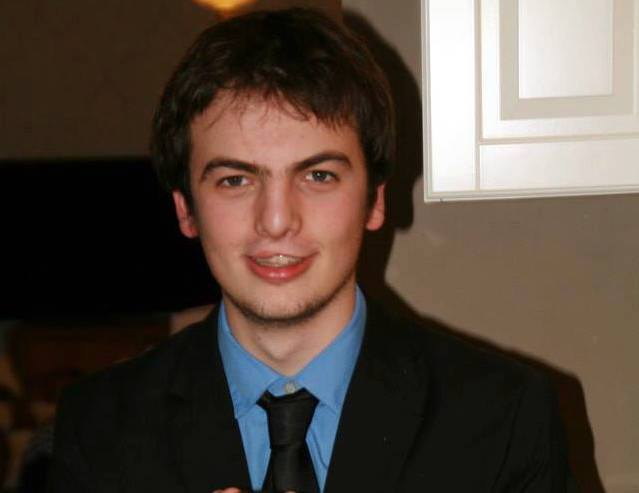
\includegraphics[scale=.2]{loic.jpg} } \vphantom{p\^{E}}}}}}
    \end{shaded}
  }\vspace{-5pt}

\end{textblock}
\begin{textblock}{10.7}(9.25, 5.5)
\resheading{Education}


\begin{itemize}
\item \ressubheading{Karlsruher Institut für Technologie}{Erasmus in the Electrical Engineering faculty}{fall 2017}
\item \ressubheading{Université Catholique de Louvain}{Master in Mathematical Engineering}{2016 - present}
\item \ressubheading{Université Catholique de Louvain}{Bachelor in Civil Engineering -  with great honor}{2013 - 2016}
\begin{itemize}
	\resitem{Specialisation in Applied Mathematics and \\ Electrical engineering}
\end{itemize}

\item \ressubheading{Martin V High School}{Graduated - with great honor}{2007 - 2013}

\end{itemize}

%%%%%%%%%%%%%%%%%%%%%%%%%%%%%%
\resheading{Professional\,Experiences}
%%%%%%%%%%%%%%%%%%%%%%%%%%%%%%



\begin{itemize}
  \item \ressubheading{Tutor in physics, chemistry and mathematics}{I gave educational support to 1st year engineering students.}{2016}
 \item \ressubheading{Tutor in physics}{I gave educational support to 1st year engineering students.}{fall 2015}
\end{itemize}

\resheading{Leisure\,Interests}
%%%%%%%%%%%%%%%%%%%%%%%%%%%%%%
\begin{itemize}
  \item \ressubheading{Chief of a scout group}{In charge of the entertainment of 36 children from 6 to 11.}{2012-2016}
 \item \ressubheading{Drummer in a band}{Creator and member of The Callaways.}{2010-2015}
  \end{itemize}

\resheading{Achievements}

\begin{itemize}
\item \begin{tabular*}{4in}{l@{\cftdotfill{\cftsecdotsep}\extracolsep{\fill}}r}
		\textcolor{mainblue}{\textbf{Belgian finale of the Emergenza festivale}} & \textit{2015} \\
		\textit{As a member of The Callaways, I performed on the multiple } &  \\
		\textit{ rounds of the Emergenza festival until the finale taking place } & \\
		\textit{at Botanique - Orangerie in Brussels.}
\end{tabular*}\vspace{-6pt}

%\item \ressubheading{Online courses}{Attented online courses}{}
%\begin{itemize}
%\item Paradigms of Computer Programming - Fundamentals (edx)
%\item Paradigms of Computer Programming - Abstraction and Concurrency (edx)
%\end{itemize}
\end{itemize}

\end{textblock}




\end{document}



